\documentclass[conference]{IEEEtran}
%Template version as of 6/27/2024

\usepackage{cite}
\usepackage{amsmath,amssymb,amsfonts}
\usepackage{algorithmic}
\usepackage{booktabs}
\usepackage{graphicx}
\graphicspath{{images/}}
\usepackage{textcomp}
\usepackage{xcolor}
\def\BibTeX{{\rm B\kern-.05em{\sc i\kern-.025em b}\kern-.08em
    T\kern-.1667em\lower.7ex\hbox{E}\kern-.125emX}}
% \setlength{\parskip}{0.8em}
\begin{document}

\title{Neural Networks for Neural Tumors\\
\vspace{-0.6em}
{\footnotesize Final Project for \textit{ECS 171 - Machine Learning} at UC Davis, with Professor Setareh Rafatirad}
}

\author{
\centering
\begin{minipage}[t]{0.9\textwidth}
  \centering
  \begin{tabular}{ccc}
    Joe Vogel & Nam Nguyen & Jonathan Mo \\
    \textit{UC Davis Computer Science} & \textit{UC Davis Computer Science} & \textit{UC Davis Computer Science} \\
    jvogel@ucdavis.edu & ncnng@ucdavis.edu & jtnmo@ucdavis.edu \\
    \vspace{0.2em}
  \end{tabular}
  \vspace{-0.6em}
  \begin{tabular}{cc}
    Aryan Karnwal & Richard Ho \\
    \textit{UC Davis Computer Science} & \textit{UC Davis Computer Science} \\
    akarnwal@ucdavis.edu & rdho@ucdavis.edu \\
  \end{tabular}
\end{minipage}
}

\maketitle

\begin{abstract}
This report documents the process of creating a machine learning model that classifies brain tumors given MRI brain scan imagery. This project saw the creation of three successful models using the following algorithms: Convolutional Neural Network, Support Vector Machine, and Random Forest. Disclaimer: this project is for educational purposes only and not meant for medical use or research.
\end{abstract}

\begin{IEEEkeywords}
Brain tumor classification, Convolutional Neural Network (CNN), MRI brain imagery, Random Forest (RF), Support Vector Machine (SVM). 
\end{IEEEkeywords}

\large 
\section{\large Introduction (Complete)}

As a team of five young computer science students with no prior machine learning experience, we ambitously decided to tackle the real world challenge of brain tumor classification. Through hours and hours of research and trial and error, we learned a lot, and we have a lot to share. 

We hope this report serves not only as an informative summary of our findings, but also as motivation for your own projects. We faced many challenges during this project, but in the end created something we are all very proud of, despite our lack of experience.

\subsection{\large Motivation}

As of 2025, there are more than 120 different kinds of brain tumors\textsuperscript{1}. Population statistics gathered by braintumor.org from 2015 through 2019 led researchers to estimate that in 2023, over 94,000 people would be diagnosed with a primary brain tumor\textsuperscript{2}, in America alone. 

Luckily, 72\% of primary brain tumors are benign. While not completely harmless, benign tumors are much less fatal than malignant (cancerous) tumors. However, that still leaves a concerning 28\% of tumors that are malignant. Of those 28\%, an estimated 65\% of cases are proven to be fatal. Among the malignant tumors, glioblastoma is the most common, with a survival rate of only 6.9\%. These numbers are tragic, and at the moment, the best way we know to reduce them is through early detection.

Hundreds of thousands of MRI brain scans are performed every day. With the scans being so intricate, it can sometimes be hard for even a trained professional to determine whether or not a patient has a brain tumor, and even harder to tell which kind. 

A tool that could detect and identify brain tumors within seconds, and with high accuracy, would not only save a lot of time and money, but lives. Like mentioned above, early detection is absolutely key to increasing survival rates. Getting more people in and out of MRI machines and having their scans be automatically processed and analyzed would save countless lives. Not to mention the impact such a tool would have on developing nations who might not have as many specially trained doctors that can readily perform MRI analysis. Luckily in the real world, hospitals are already adopting and developing these ideas. 

\subsection{\large Approach}

A classification machine learning model is a great approach to this problem. Using a convolutional neural network and an image dataset, we can train a model to accuractely classify brain tumors. With its complex structure, a CNN can detect nuances and patterns in the scans that are otherwise hard to spot. 

This project focuses on three general brain tumor classes: glioma, meningioma, and pituitary. Each class contains many of the 120+ tumor types mentioned before. The model will also have a "no tumor" class. The aim for the model was to predict tumor classes with over 95\% accuracy.

\section{\large Literature Review (Complete)}

\subsection{\large Brain Tumor Classification in MRI Image Using Convolutional Neural Network\textsuperscript{3}}

In this article from 2021, authors Khan et al. examine convolutional neural network models for brain tumor classification, reporting classification accuracies ranging from 80\% to 98\%. The authors highlight two primary challenges in training such models: (1) the scarcity of accurately labeled data, which increases training complexity and cost, and (2) inconsistency in image dimensions, given that CNNs require fixed-size input. Their dataset is partitioned into training, validation, and testing sets, serving model training, hyperparameter tuning, and final evaluation, respectively. Image pre-processing is performed using Canny Edge Detection, an open-source computer vision technique. To address the limited dataset size, the authors employ data augmentation methods such as flipping, rotation, and brightness adjustments to enhance variability. The model utilizes the ReLU activation function and stochastic gradient descent for optimization.

Given our limited computational resources, we plan to utilize a pre-trained model. The eight-layer architecture discussed in the paper provides a useful baseline. The pre-processing techniques mentioned are also great starting points for us, and let us know what we should look out for. Furthermore, we intend to implement data augmentation techniques to improve generalization on our small dataset. The use of ReLU and stochastic gradient descent aligns well with our current understanding, and we aim to assess their impact on our model's performance.

\subsection{\large A Deep CNN Based Multi-Class Classification of Alzheimer's Disease Using MRI\textsuperscript{4}}

In this article, Farooq, Anwar, Awais, and Rehman demonstrate their implementation of a four-way Alzheimer's disease classifier. Considering their model also takes MRI imagery as input and has four class target labels, we can learn a lot from their experiments. The authors began their model development with data preprocessing and a technique known as skull stripping, which is the process of removing non-brain tissues like the skull or fat from MRI imagery. We could implement skull stripping in our model to improve the signal-to-noise ratio and reduce input complexity, which could help against overfitting. 

Additionally, the article mentions the utilization of data augmentation to increase the data set; they simply flipped the images along the horizontal axis, which is valid due to the left and right symmetry of the brain. This method increased their dataset from 355 MRI volumes to 38024 images. We can implement the same method in our project because increasing the sample size can combat overfitting, making our model more accurate.

\subsection{\large Brain Tumor Classification Using Convolutional Neural Networks\textsuperscript{5}}

In this publication, authors Seetha and Raja demonstrate the effectiveness of convolutional neural networks for brain tumor classification. Their proposed CNN-based classification approach achieves an impressive 97.5\% accuracy rate while maintaining low computational complexity compared to other methods. Seeing such a high accuracy be achieved is both inspiring and motivating for us. Considering their model also predicts four tumor types, their high accuracy rate sets a benchmark we should aspire to, and their focus on computational efficiency aligns with our resource constraints. 

The authors implemented a deeper architecture design using small kernels, with neuron weights intentionally kept small to optimize performance. Their experimental results demonstrated that their CNN model outperformed other state-of-the-art methods in both accuracy and efficiency. Like our approach, they used a dataset containing various brain MRI scans and faced similar challenges with image preprocessing. Their optimization of kernel size and weight parameters offers valuable insights for our model development. Given that our initial prototype showed signs of overfitting (93\% training accuracy with 42\% testing accuracy), we should consider implementing some of the suggested architectural decisions regarding smaller kernels and weight optimizations, while continuing with our planned transfer learning approach to improve generalization.

\section{\large Dataset Description (Complete)}

The dataset used for this project comes from a group of brilliant students at Savitribai Phule Pune University in India. It is an open source dataset that can be found for free on Kaggle\textsuperscript{6}. The dataset is reviewed and well respected. It consists of 3264 labeled MRI scan images. Like hinted at before, the images are divided into four categories: three different tumor types, and one set of “no tumor” scans. Because each image in our dataset is already labeled, our model's training is considered supervised, as opposed to unsupervised. An unsupervised model would require a much different approach, most likely using different algorithms.

\subsection{\large Preprocessing}

Due to the non-numerical nature of image datasets, our input features come in a different form than they normally would with a numerical dataset. Instead of having numerically represented features such as 'age', 'blood pressure', and so on, our dataset only has images. Technically, each image is a set of numbers (pixel intensities), but the idea remains. There is no standard feature selection process, or process to choose which features to train the model on. Instead, things like image preprocessing and model hyperparameters are key to training an accurate model.

As explained under 'Literature Review', preprocessing steps might include techniques like image resizing, cropping, normalization, data augmentation (rotating, flipping, zooming), and more. Going even further, the 'skull stripping' technique mentioned by Farooq et al.\textsuperscript{4} can be used to isolate the brain tissue in an MRI scan. This is helpful for training a model, since we do not care about the skull or fat in the scans, it is considered noise. We do not want the model to train on those "features" of the image.

\section{\large Exploratory Data Analysis (1 page)}
% TODO: Complete but need to fix image placement so that EDA is on one consistent page

% EXAMPLE image in a column
% \begin{figure}[!ht]
%     \centering
%     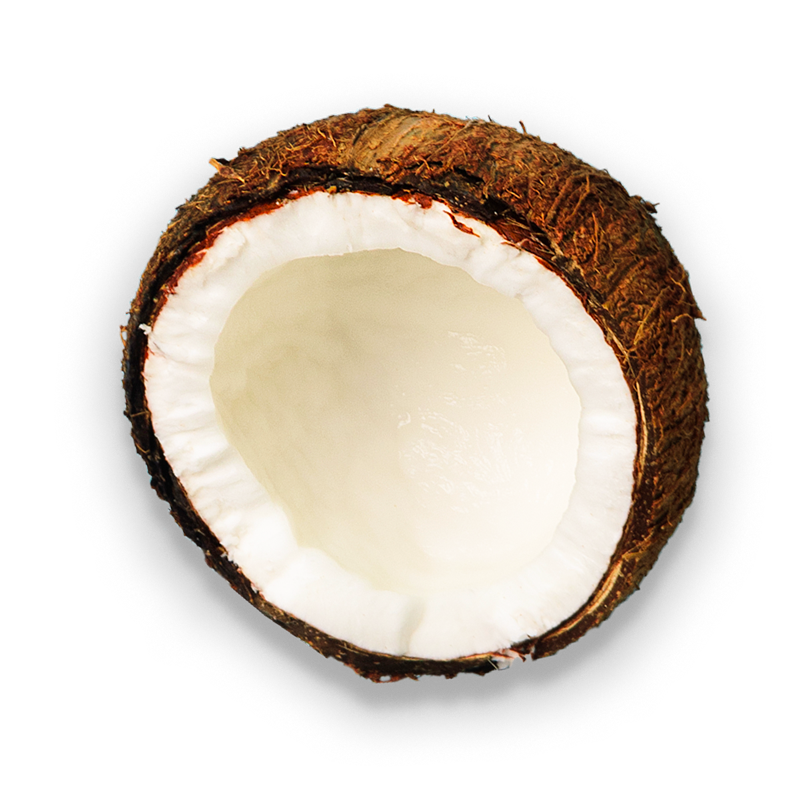
\includegraphics[width=2in]{coconut.png}
%     \caption{this is a coconut}
%     \label{test image coconut}
% \end{figure}

% EXAMPLE image across two columns
% \begin{figure*}[!ht]
%     \centering
%     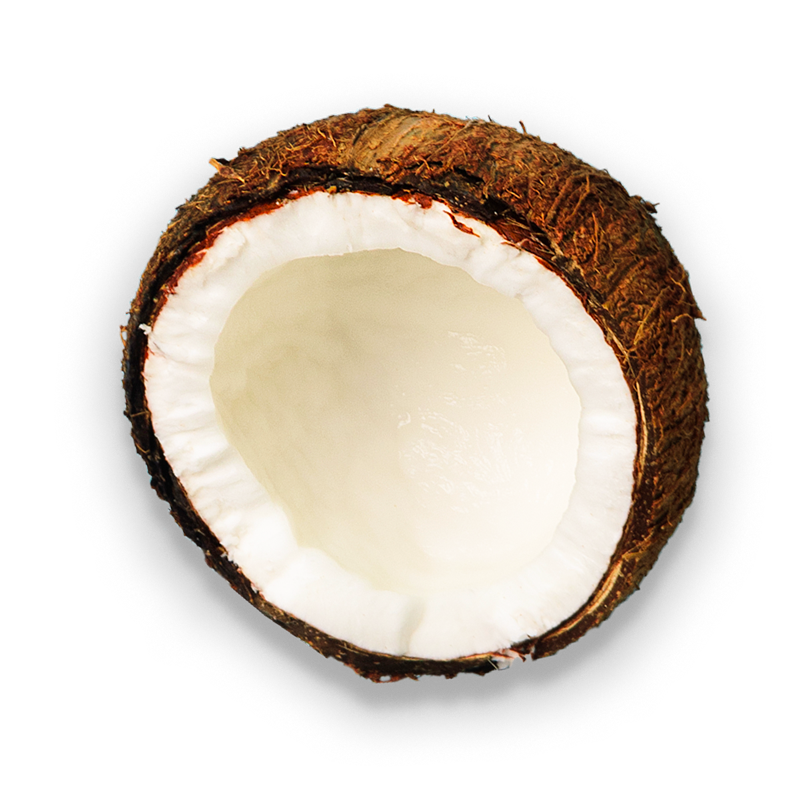
\includegraphics[width=3in]{coconut.png}
%     \caption{this is a coconut}
%     \label{coconut}
% \end{figure*}

% These two won't stay in the same row
% \begin{figure*}[!ht]
%     \centering
%     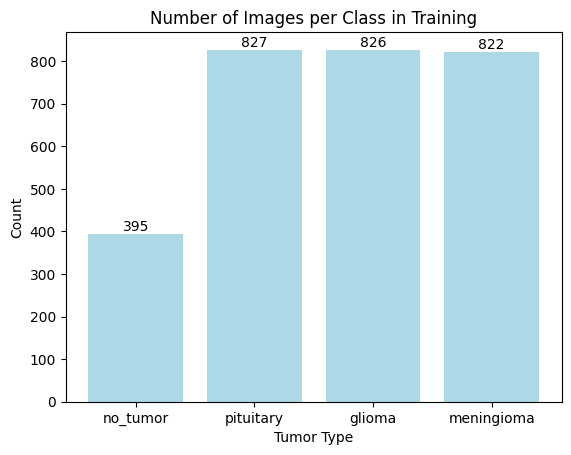
\includegraphics[width=1in]{ImagesPerClassTraining.png}
%     \caption{\large Images in the training dataset}
%     \label{Number of images per class in the training dataset}
% \end{figure*}

% \begin{figure*}[!ht]
%     \centering
%     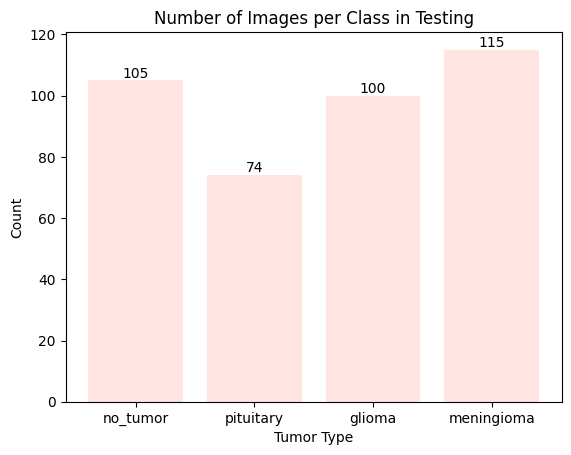
\includegraphics[width=1in]{ImagesPerClassTesting.png}
%     \caption{\large Images in the testing dataset}
%     \label{Number of images per class in the testing dataset}
% \end{figure*}

% Both figures in one row
% TODO: Move these to be under EDA in the right spots
\begin{figure*}[!ht]
    \centering
    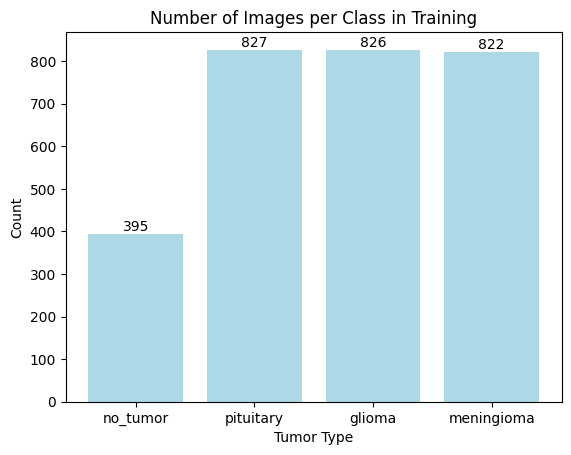
\includegraphics[width=0.49\textwidth]{ImagesPerClassTraining.png}
    \hfill
    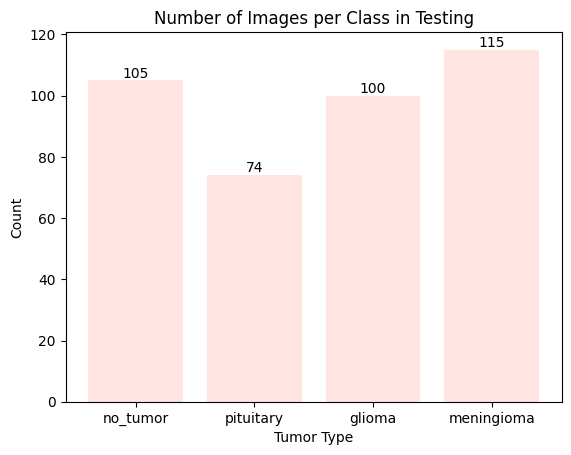
\includegraphics[width=0.49\textwidth]{ImagesPerClassTesting.png}
    \caption{\large The dataset has a consistent number of training images across classes, except for "no tumor". This should not be an issue because "no tumor" imagery has much less variance. For testing, the distribution of images is more varied, but this does not affect model performance, since the model is not trained on this data.}
    \label{images-per-class}
\end{figure*}

As seen in the left histogram of \textit{Figure 1}, there is a relatively even distribution of data among each class in the training set, at around 825 images. However, the no tumor class has significantly less, with 395 images. We suspect this is because the scans without tumors have much less variance. And because of the reduced variance, it should be much easier for the model to detect "no tumor" scans. We did not think the lower number of images would have a negative effect on the model's ability to classify images as "no tumor", and we were right. However, if we did see poor results in that classification specifically, we could have tried training the model on 395 images for each class to see if that helped with the overfitting of the other classes. On the other hand, we could have performed data augmentation on the "no tumor" class, bringing its number of images up to the 825 range like the other classes. In hindsight, we did not have to apply either of these techniques.

Shifting our focus toward the testing dataset, again looking at \textit{Figure 1}, but this time at the right histogram, we see that there is a much more uneven distribution among each class. This does not affect our model's performance, since it is not being trained on the testing data. However, we thought the results of the pituitary class could be skewed considering the relatively low number of pituitary, but it was also not a problem. If we had seen inconsitencies, it could have been useful to test against more pituitary imagery to ensure the model can handle all variations of scans. We could again have performed data augmentation to create more pituitary data. Testing against more data could give us more confidence in our model.

\begin{figure*}[!ht]
    \centering
    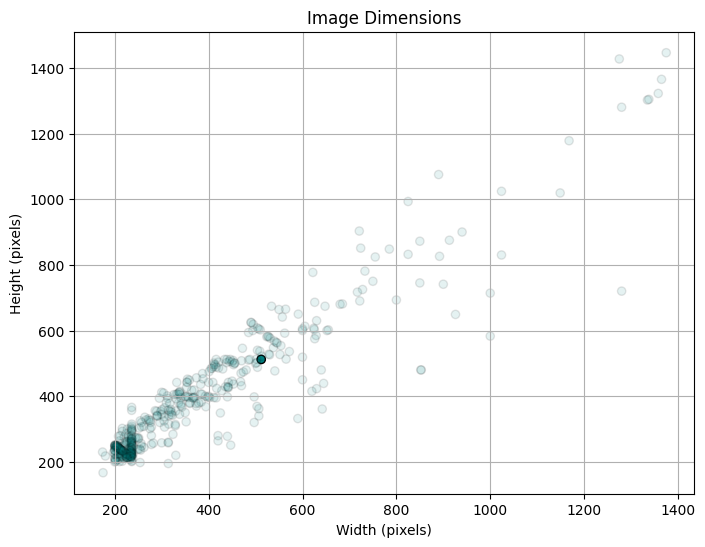
\includegraphics[width=5in]{ImageDimensions.png}
    \caption{\large It is clear to see the images in the dataset are of many varying dimensions. We do see higher densities around the 200x200 and 500x500 dimensions, though. Regardless, such variation means image preprocessing and resizing is necessary before training.}
    \label{Dimensions of images in the dataset}
\end{figure*}

Taking a look at Figure 2, we can see that the dataset is comprised of images of many varying sizes. There is a concentration around the 200x200 and 500x500 sizes. With this information, we know we will have to perform some image pre-processing to convert all images into the same size so the model has consistent input. 

\section{\large Methodology (Complete)}

\subsection{\large Feature Selection}

As mentioned in the dataset description, we don't have labels for our input features like a numerical dataset would have. We only have our images, which are technically each a set of pixel intensity values, but it means we can't select certain features to train our model on. Instead, we can perform some image preprocessing and hyperparameter tuning to increase our model's accuracy.

Looking at Figure 2 again, we see all of our images have different dimensions. As a preprocessing step, we will resize all images to be 224x224 pixels, the conventional CNN input size. The resizing step is not as simple as it sounds though, we must be careful not to create unwanted noise in our data. After imagine resizing, we then normalize each pixel's value from its 3-channel RGB form.

The training dataset consists of 2870 MRI scans. To increase the size of the training dataset, we can perform data augmentation like mentioned previously. We can rotate, flip, and zoom the images to create `artificial' data that would hopefully reduce any overfitting and allow for the model to better capture underlying patterns. We also would expect this technique to allow for the model to predict against a larger variety of testing data (i.e. rotated images). 

Along with input features, the hyperparameters of a model are crucial to achieving a good fit. The key hyperparameters for the CNN model were: batch size for gradient descent, training epochs, loss function, dropout rate, and a few others. We used grid search to find optimal parameters for all three of our models, more on that later. 

\subsection{\large Early Model Development}

Our first prototype model was a CNN with four convolutional blocks, followed by fully connected layers using the Keras Sequential API. We trained the model over 20 epochs, with each epoch giving us higher accuracy on the training data, peaking at 93\%. However, when performing predictions on our testing data, the model saw a big dip in performance. With an average accuracy of 42\%, we knew immediately that our model was heavily overfitting the training data.

To improve upon the first model, we applied k-fold cross validation and tuned hyperparameters such as dropout rate, number of layers, number of neurons, etc. This was the first time we used grid search to tune hyperparameters. It was also at this stage we decided that going forward, we would use transfer learning to reduce the number of learned parameters and implicitly filter irrelevant `features'. Transfer learning, which is the process of leveraging a pre-trained model to improve your own, can greatly reduce overfitting risks. From this point on, we used PyTorch. Pytorch gave us more flexibility in controlling forward pass, backpropagation, and optimization, allowing us to develop a better-fitting CNN model.

\section{\large Experimental Results (Complete)}

Neural networks like CNNs are very good at detecting features and learning patterns in data. Because of this, we can leverage deep learning to preprocess data, and then use that data to train other models. So far, this report has focused on developing a CNN model with high accuracy by iteratively refining both model architecture and training strategy. While CNNs are the most common algorithm choice for image classification, they are not the only option. Image classification can be done by various other algorithms, including support vector machine (SVM), and random forest (RF). 

While the detailed performance of each model we created will be discussed in the following sections, this section outlines the chronological development and iterative experimentation that lead us to our final models.

\subsection{\large Baseline CNN Model}

Like mentioned before, our very first model was built from scratch using TensorFlow's Sequential API. The model consisted of four convolution blocks with subsequent increases in the number of filters (kernels). Each block was followed by a max pooling layer helping reduce the spatial dimensionality. Additionally, each hidden layer of the model was accompanied by a dropout layer to mitigate overfitting. The last hidden layer of the model was a dense layer of 128 neurons using the ReLU activation function. The output layer was four neurons using Softmax as the activation function. Softmax, given its consistent output between 0 and 1, is the standard choice of activation function for the output layer in multi-class classification. 

This model was trained over 20 epochs using the Adam optimizer and categorical cross-entropy as the loss function. And as mentioned before, the model ended up with a training accuracy of 93\% and a testing accuracy of 42\%, implying significant overfitting.

\subsection{\large Transfer Learning with ResNet50}

In our next step, we decided to employ transfer learning. We started with the ResNet50 model, a pre-trained model trained on the ImageNet dataset. We leveraged the architecture of ResNet50 as a feature extractor by eliminating its output layer and freezing all other layers. The classification head was built on top of the pre-trained model, which served as a convolutional base. The base was followed by a Global Average Pooling layer to compress spatial dimensions. The classifier was again completed by a fully connected dense layer of 128 neurons with the ReLU activation function and a Softmax output layer. The layer of 128 neurons was accompanied by a dropout rate of 0.3 to help prevent overfitting.

The model was trained over 20 epochs. The transition to transfer learning yielded a significant improvement in validation accuracy (89\% compared to 76\% in the first model) while maintaining a reasonable training accuracy of 93\%. Motivated by this encouragement, we experimented with selective fine-tuning the model by unfreezing the last 30 layers of the ResNet50 pre-trained model, allowing the weights of those layers to be adjusted during backpropagation. With this adjustment, the model ended up with a training accuracy of 97\%, and a testing accuracy of 79\%. Although the model was still slightly overfitting, we had made huge improvements. At this stage, we also introduced new training practices such as the learning rate hyperparameter and early stopping, which shaped our training strategy for later experiments.

\subsection{\large Dataset Reorganization and ResNet101 Upgrade}

Motivated by the significant improvement in the previous stage, we had defined that transfer learning would be one of the most critical techniques in developing our CNN model. We decided to try different pre-trained models, from simpler models such as VGG16 and VGG19, to more complex ones in the ResNet and EfficientNet families. Even with either layer-wise fine-tuning or standard fine-tuning techniques applied to those models, we had noticed a common trait, persistent underperformance on the testing test (with an accuracy around 70\% to 80\%). This discrepancy prompted us to re-evaluate our dataset. Initially, we had used the dataset split provided by Kaggle. We suspected that there might have been an imbalanced presentation across classes or feature distribution in the default split. To resolve this issue, we decided to recombine the training and testing sets with shuffle, then split the entire dataset with a ratio consistent with that of the default split.  

With limited available computational resources, we also upgraded our pre-trained model to ResNet101, a more complex model compared to ResNet50. We employed the same structure as in the ResNet50 setup. The model was initially trained over 20 epochs with all ResNet101 layers frozen, yielding a training accuracy of 92\% and validation accuracy of 85\%. When the fine-tuning technique was applied (with the last 40 layers unfrozen), the model reached 99\% training accuracy and 96\% validation accuracy after being trained over four additional epochs. The model also performed much better on the testing data, yielding 97\% accuracy with reasonably high f1-scores for each class label. This was our breakthrough.

By employing ResNet101 with layer-wise fine-tuning and a better dataset split, we ended up with a highly robust CNN model with consistent performance across training, validation, and testing data.

\subsection{\large Non-deep Learning Models with feature extraction}

To develop other classifiers that incorporate algorithms rather than deep learning, we decided to employ Support Vector Machine (SVM) and Random Forest (RF) models. We leveraged the fine-tuned CNN model as the feature extraction for our selected dataset in order to obtain high accuracy while keeping the training process relatively simple. More specifically, we extracted the output of the GlobalAveragePooling2D layer of the fine-tuned CNN model, which includes 2048-dimensional feature vectors, and that result would serve as the input for each non-deep learning model. In other words, our SVM and RF models were trained on a more semantically meaningful input space compared to raw pixels. 

After conducting hyperparameter tuning, we obtained an overall accuracy of 96\% and 95\% for SVM and RF classifiers respectively. In general, these results demonstrate that classical classifiers, when paired with feature extractors, can deliver highly competitive performance for image classification, with significantly reduced training complexity.

\section{\large Evaluation (1-2 pages)}

\begin{table}[h!]
\centering
\caption{CNN Metrics}
\begin{tabular}{lcccc}
\toprule
\textbf{Class} & \textbf{Precision} & \textbf{Recall} & \textbf{F1-score} & \textbf{Support} \\
\midrule
glioma     & 0.98 & 0.93 & 0.95 & 109 \\
meningioma & 0.93 & 0.97 & 0.95 & 105 \\
no tumor   & 0.97 & 0.98 & 0.98 & 60 \\
pituitary  & 0.99 & 0.99 & 0.99 & 118 \\
\midrule
\textbf{Accuracy} \textbf{0.97} \\
\bottomrule
\end{tabular}
\end{table}

\begin{table}[h!]
\centering
\caption{SVM Metrics}
\begin{tabular}{lcccc}
\toprule
\textbf{Class} & \textbf{Precision} & \textbf{Recall} & \textbf{F1-score} & \textbf{Support} \\
\midrule
glioma     & 0.98 & 0.91 & 0.94 & 109 \\
meningioma & 0.89 & 0.97 & 0.93 & 105 \\
no tumor   & 0.98 & 0.97 & 0.97 & 60 \\
pituitary  & 0.98 & 0.98 & 0.98 & 118 \\
\midrule
\textbf{Accuracy} \textbf{0.96} \\
\bottomrule
\end{tabular}
\end{table}

\begin{table}
\centering
\caption{RF Metrics}
\begin{tabular}{lcccc}
\toprule
\textbf{Class} & \textbf{Precision} & \textbf{Recall} & \textbf{F1-score} & \textbf{Support} \\
\midrule
glioma     & 0.98 & 0.89 & 0.93 & 109 \\
meningioma & 0.87 & 0.98 & 0.92 & 105 \\
no tumor   & 1.00 & 0.93 & 0.97 & 60 \\
pituitary  & 0.97 & 0.98 & 0.98 & 118 \\
\midrule
\textbf{Accuracy} \textbf{0.95} \\
\bottomrule
\end{tabular}
\end{table}

In this project, three machine learning models—Convolutional Neural Networks (CNN), Support Vector Machines (SVM), and Random Forests (RF)—were trained and evaluated. In this section, the performance of these models are assessed using standard classification metrics, including accuracy, precision, recall, and F1 score. The dataset utilized for this evaluation consists of four classes: glioma, meningioma, pituitary tumor, and no tumor.

The CNN model demonstrated the highest overall accuracy at 96.68\%, followed closely by SVM at 95.66\%, and RF at 94.90\%. Macro and weighted F1-scores mirrored this trend, with CNN achieving 0.97, SVM 0.96, and RF 0.95 in both averages. These scores indicate that CNN not only achieves better overall classification performance but also maintains consistency across classes in terms of precision and recall.

Diving into per-class specifics, we observe that for the label "glioma", CNN exhibited the highest precision (0.98) and recall (0.93), indicating strong identification capability with few false positives and a relatively low false negative rate. SVM matched CNN in precision (0.98) but had a lower recall (0.91), while RF also had a precision (0.98) but the lowest recall score at 0.89. This suggests that both SVM and RF are more likely to miss "glioma" cases compared to CNN while matching its precision.

In the case of "meningioma", while CNN had the best precision (0.93), SVM and RF had equal or superior recall (0.97 and 0.98 respectively) compared to CNN (0.97). SVM and RF had reduced precision (0.89 and 0.87) which is a notable difference from CNN's aforementioned score. This pattern indicates that SVM and RF are more sensitive in detecting "meningioma" but may yield more false positives than CNN.

In classifying "no tumor", RF achieved perfect precision (1.00), which means that every time RF predicted "no tumor", the model was correct. However, its recall (0.93) was the lowest among the three, pointing to a higher rate of false negatives. CNN balanced both precision (0.97) and recall (0.98) well, outperforming both alternatives in overall reliability for this class.

For the label 'pituitary', all three models performed strongly, with CNN leading both in precision and recall (0.99 each). SVM and RF followed closely with both metrics at 0.98 and 0.97-0.98, respectively, indicating that all models are highly effective in classifying "pituitary" tumors.

Unlike accuracy, which can be misleading if one class dominates the dataset, the F1 score provides a balanced view of the model's ability to correctly identify each class without favoring either false positives or false negatives. This makes it especially useful in medical imaging applications, where both types of errors can have serious implications for patient diagnosis and treatment.

The F1 score of 0.93 for glioma tumors. This score indicates that while the model performs well in identifying glioma cases, there is a notable trade-off between precision and recall, particularly with slightly reduced recall. This suggests the model may occasionally misclassify glioma tumors as other types or miss them altogether.

The meningioma class has the lowest F1 score among all four classes with 0.92, indicating the greatest challenge for the model in this category. The score suggests a less favorable balance between precision and recall; either the model is producing more false positives, false negatives, or both. This could be due to visual overlap with other tumor types, particularly gliomas, or due to greater variability in meningioma imaging features. 

The F1 score of 0.97 for the no tumor class highlights the model’s strong performance in distinguishing healthy scans from non-healthy ones. The high precision and recall underlying this score indicate that the model rarely misclassifies healthy brains as tumors meaning there are a low amount of false positives and is also unlikely to miss the absence of a tumor or false negatives. This reliability is crucial in medical settings, where a false alarm can lead to unnecessary procedures, and a missed tumor can be life-threatening.

With the highest F1 score of 0.98, the model shows excellent performance in detecting pituitary tumors. This suggests that the pituitary tumor class is the most distinct or consistently represented in the dataset, allowing the model to make confident predictions. High F1 scores for both precision and recall indicate that pituitary tumors are both correctly identified and rarely confused with other classes. This robustness may stem from more uniform imaging patterns or stronger contrast features in this tumor type.

\section{\large Conclusion (1/2 page)}

The above evaluation highlights CNN's strength in handling complex, high-dimensional image data, likely due to its hierarchical feature extraction capability. Its superior balance in both precision and recall in all tumor types supports its suitability for real-world clinical deployment, where false positives and false negatives carry significant risk.

SVM performed comparably well, especially in the detection of meningioma and pituitary tumors, and may offer a lighter alternative in environments with limited computational resources. However, it showed reduced precision in some classes, which made it slightly less robust overall.

RF, while achieving remarkable precision, particularly for the "no tumor" class, exhibited reduced recall across multiple classes. This suggests a tendency to make fewer false positives, at the expense of missing actual tumor cases, which is a very serious and life-threatening issue in medical diagnostics.

\section{\large Our Team (1 page)}

The link to this project's GitHub\textsuperscript{10} repository can be found in the references of this report. The repository holds our source code, the dataset, this report, and some more supplementary files. Please feel free to fork the repository and mess around with it as you wish.

Project roadmap? Reference the first one pager outline assignment we did on google doc
%TODO --- roadmap?

\subsection{\large Demonstration}

For those interested in seeing the model in action, a short five minute demonstration of our model can be found on YouTube\textsuperscript{11}. The demo briefly walks through how to use the model, how the frontend was developed, and how the model is invoked.

\subsection{\large Roles and Contributions}

Joe: As the team leader, Joe took charge of logistics. He organized meetings, defined the roadmap for the project, and kept the team on track. He also lead the exploratory data anaylsis subproject, and was crucial to the creation of the final report. 

Nam: Throughout the progression of the project, Nam was primarily responsible for the development and implementation of machine learning models. 
Nam took over the experimental process to optimize each model, iteratively researching multiple architectures and frameworks to successfully develop models with different algorithms that are able to perform brain tumor detection at a relatively high accuracy. 
In general, Nam’s contributions encompassed every stage of model development, from initial prototyping to completion of each model prior to final deployment, ensuring both technical robustness and adaptability to team-driven refinements.

Jonathan: Jonathan took charge of literature review and researched techniques that can be implemented to the model. Jonathan was also responsible for writing the evaluation section that analyzed the performances of the models by talking about the evaluation metrics such as F1 scores, precision, and recall across the different classes. 

Richard: Richard contributed to the project by evaluating the performance of the three machine learning model using evaluation metrics such as accuracy, F1 score, precision, and recall. Based on these analyses, he provided the rationale for selecting the CNN model as the final model due to its superior performance relative to the alternatives. Additionally, he conducted a comprehensive literature review to summarize key developments in the field, which served as a foundational reference for the project. His contributions also included performing exploratory data analysis (EDA) and preparing the dataset for modeling through appropriate data preprocessing techniques.

Aryan: Aryan participated in group meetings, worked on literature reviews, helped the group brainstorm ideas and find the dataset, built and deployed the fullstack application, and created the demo video. 

\begin{thebibliography}{00}

\bibitem{Hopkins2025}
Brain tumor types. Johns Hopkins Medicine. (2021, November 8). https://www.hopkinsmedicine.org/health/conditions-and-diseases/brain-tumor/brain-tumor-types 

\bibitem{NBTS2022}
Brain tumor facts. National Brain Tumor Society. (2024, February 20). https://braintumor.org/brain-tumors/about-brain-tumors/brain-tumor-facts/ 

\bibitem{Khan2021}
H. A. Khan, W. Jue, M. Mushtaq, and M. U. Mushtaq, “Brain tumor classification in MRI image using convolutional neural network,” *Math. Biosci. Eng.*, 2021. 

\bibitem{Farooq2017}
A. Farooq, S. Anwar, M. Awais, and S. Rehman, “A deep CNN based multi-class classification of Alzheimer's disease using MRI,” in *Proc. IEEE Int. Conf. Imaging Syst. Tech. (IST)*, 2017, pp. 1-6. 

\bibitem{Seetha2018}
J. Seetha and S. S. Raja, “Brain tumor classification using convolutional neural networks,” *Biomed. Pharmacol. J.*, vol. 11, no. 3, p. 1457, 2018.

\bibitem{Sartaj2020}
Sartaj. “Brain Tumor Classification (MRI).” Kaggle, 24 May 2020, www.kaggle.com/datasets/sartajbhuvaji/brain-tumor-classification-mri. 

\bibitem{Kumar2014}
R. S. Kumar and M. Karnan, “Review of MRI image classification techniques,” *Int. J. Res. Stud. Comput. Sci. Eng.*, vol. 1, no. 1, pp. 21-28, 2014. 

\bibitem{Hasan2019}
A. M. Hasan, H. A. Jalab, F. Meziane, H. Kahtan, and A. S. Al-Ahmad, “Combining deep and handcrafted image features for MRI brain scan classification,” *IEEE Access*, vol. 7, pp. 79959-79967, 2019. 

\bibitem{Meier2020}
R. Meier, A. P. de Mortanges, R. Wiest, and U. Knecht, “Exploratory analysis of qualitative MR imaging features for the differentiation of glioblastoma and brain metastases,” *Front. Oncol.*, vol. 10, p. 581037, 2020.

\bibitem{Vogel2025}
J. Vogel, N. Nguyen, J. Mo, A. Karnwal, R. Ho, "Neural Networks for Neural Tumors". GitHub. https://github.com/Coco501/Neural-Networks-
for-Neural-Tumors

\bibitem{Karnwal2025}
A. Karnwal, "Brain Tumor Classification Application Demo". (2025), YouTube. https://www.youtube.com/watch?v=ECMGXgMrji0

\end{thebibliography}


\end{document}
